\documentclass[a4paper, 12pt]{article}

\usepackage{utils}

\pgfplotsset{width=10cm,compat=1.9}

\renewcommand*{\today}{19 septembre 2024}

\begin{document}

\hotbox{Analyse 1}{CM 3}{\today}

\subsection{Propriété d'Archimède}

L'ensemble $\R$ est dit archimédien, i.e. $\forall x \in \R, \exists n \in \N, \; x \lt n$

\begin{proposition}{}{}
    Il existe un unique entier dans $\Z$, appelé la partie entière E, tel que $E(x) \leq E(x) + 1$
\end{proposition}

\begin{demonstration}
    \textbf{Existence:} Supposons que $x \geq 0$.
    Comme $\R$ est archimédien il existe un entier $n \in \N$ tel que $x \lt n$.

    Ainsi on peut trouver un autre entier $m \in \N$ tel que $n \leq x$ et $m \lt n$.
    Il suffit de choisir m comme le plus grand entier inférieur ou égal à x et tel que $m \leq x \lt m + 1$

    \vspace{1em}

    \noindent
    \textbf{Unicité:} Supposons qu'il existe 2 entiers tel que $k \leq x \lt k + 1$ et $l \leq x \lt l + 1$

    Par transitivité, il vient $k \leq x \lt l + 1$ et $k \lt l + 1$,

    de même, $l \leq x \lt k + 1$ et $l \lt k + 1 \implies l - 1 \lt k$

    Finalement $l - 1 \lt k \lt l + 1$ et comme entre les entiers l'entier l-1 et l+1 il n'y a que l, alors k = l
\end{demonstration}

\begin{exemple}
    \item x = 3.14, E(x) = 3.
    \item x = -12.2, E(x) = -13.
\end{exemple}

\begin{remarque}
    \item On note parfois $E(x) = [x] = \lfloor x \rfloor$
    \item On note $\{x\}$, la partie fractionnaire (e.g. $\{3.14\}=0.14$)
\end{remarque}

% \begin{tikzpicture}
%     \begin{axis}[axis lines=middle, grid]
%         \addplot[
%             jump mark right,
%             domain=-3:3,
%             samples=7,
%             very thick, red,
%         ]{floor(x)};
%         \addlegendentry{\(E(x)\)};
%     \end{axis}
% \end{tikzpicture}

% \begin{tikzpicture}
%     \begin{axis}[axis lines=middle, grid, ymin=-3, ymax=3]
%         \addplot[
%             jump mark right,
%             domain=-3:3,
%             samples=1000,
%             very thick, red,    
%         ]{x-floor(x)}; 
%         \addlegendentry{$\{x\}$};
%     \end{axis}
% \end{tikzpicture}

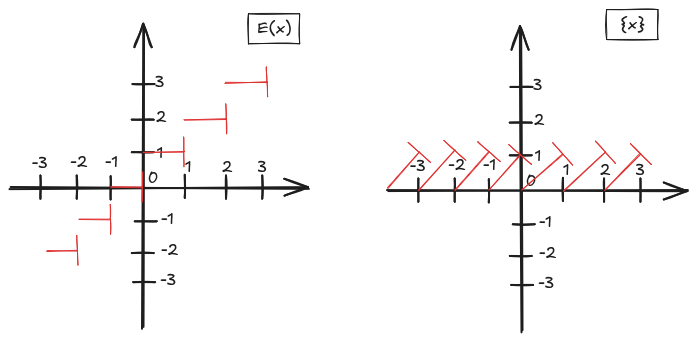
\includegraphics[width=\textwidth]{../images/Entier&fractionaire.png}

\subsection{La valeur absolue}

\begin{definition}
    Soit x un nombre réel. La valeur absolue de x est le nombre réel positif défini par
    \begin{equation}
        |x| =
        \begin{cases}
            x, & \text{si } x \geq 0 \\
            -x, & \text{si } x \lt 0
        \end{cases}
    \end{equation}
\end{definition}

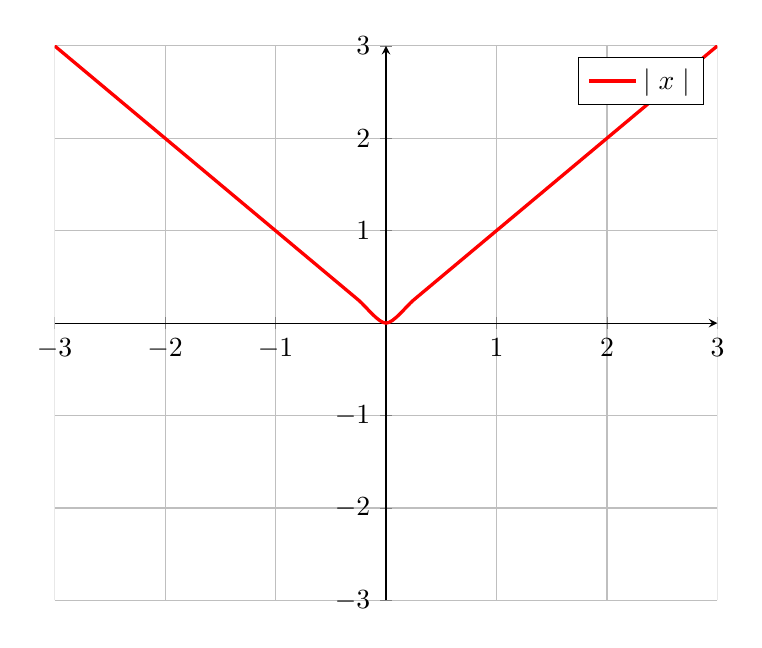
\begin{tikzpicture}
    \begin{axis}[axis lines=middle, grid, ymin=-3, ymax=3]
        \addplot[
            jump mark right,
            domain=-3:3,
            smooth,
            very thick, red,    
        ]{abs(x)}; 
        \addlegendentry{$\mid x \mid$};
    \end{axis}
\end{tikzpicture}

\noindent
Soient $a, b, c \in \R$

\begin{propriete}{}{}
    \begin{enumerate}
        \item $|a| \geq 0, \quad a \leq |a|, \quad -|a| \leq a, \quad |-a| = |a|$
        \item $\sqrt{a^2} = |a|$
        \item $|ab| = |a||b|$
        \item $\forall n \in \Z, |a^n| = |a|^n$
        \item $\text{si } a \neq 0, |\dfrac{1}{a}|=\dfrac{1}{|a|} \text{ et } |\dfrac{b}{a}| = \dfrac{|b|}{|a|}$
        \item
        $\text{Pour } b \geq 0,$
        
        $|a| = b, \text{ si et seulement si } a = b \text{ ou } a = -b$
        
        $|a| \leq b \text{ si et seulement si } -b \leq a \leq b$ (beaucoup utilisé pour passer de $a$ à $|a|$)
        
        $|a| \geq b \text{ si et seulement si } a \leq -b \text{ ou } a \geq b$
        \item $|a + b| \leq |a| + |b|$ (l'inégalité triangulaire)
        \item $||a| - |b|| \leq |a - b|$ (l'inégalité triangulaire inversée)
    \end{enumerate}
\end{propriete}

Les propriétés 1 à 6 sont démontrés par la définition de la valeur absolue

Démontrons la proprétée 7.

\begin{demonstration}
    D'après (1) \quad
    $-|a| \leq a \leq |a|$ et $-|b| \leq b \leq |b|$
    
    En additionnant, on obtient $-|a|-|b| \leq a + b \leq |a| + |b|$

    $-(|a|+|b|) \leq a + b \leq |a| + |b|$ avec (6) on arrive à

    $|a + b| \leq |a| + |b|$
\end{demonstration}

Démontrons la propriétée 8.

\begin{demonstration}
    $a = a - b + b$ \quad et \quad $|a| = |a - b + b| \leq |a - b| + |b|$ (propriétée 7)

    $|a| \leq |a - b| + |b| \implies |a| - |b| \leq |a - b|$

    \vspace{0.5em}
    de même, 
    \vspace{0.5em}
    
    $b = b - a + a$ \quad et \quad $|b| = |b - a + a| \leq |b - a| + |a|$
    
    $|b| \leq |b - a| + |a| \implies |b| - |a| \leq |b - a|$
    
    \vspace{0.5em}

    $|b - a| = |-(a-b)| = |a-b|$ et
    
    $|a| - |b| \leq |a-b|$ \quad et \quad $|b| - |a| = -(|a| - |b|) \leq |a-b|$

    Finalement par définition

    \begin{equation*}
        ||a|-|b|| =
        \begin{cases}
            |a| - |b|, & \text{si } |a| - |b| \geq 0 \\
            -(|a| - |b|), & \text{si } |a| - |b| \lt 0
        \end{cases}
    \end{equation*}
    Ainsi $||a| - |b|| \leq |a - b|$
\end{demonstration}

Corollaire: Soit r un réel positif $\forall x, a \in \R$, on a 
$|x - a| \lt r \implies -r \lt x - a \lt r \implies a-r \lt x \lt a + r$

\begin{remarque}
    La valeur absolue $|b - a|$ représent la distance entre a et b
\end{remarque}

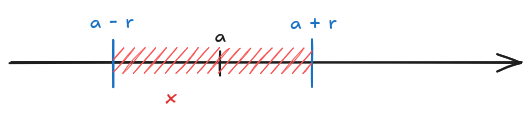
\includegraphics[width=\textwidth]{../images/neightborhood.png}

\section{Densité de $\Q$ dans $\R$}

\subsection{Intervalles de $\R$}

\begin{definition}
    On appelle intervalle de $\R$, tout sous-ensemble I de $\R$ vérifiant
    $\forall a, b \in I, a \leq b \text{ et } x \in \R, a \leq x \leq b \implies x \in I$
\end{definition}

\begin{remarque}
    Un sous-ensemble ou partie I de $\R$, se note $I \subset \R$
\end{remarque}

\begin{definition}
    Soient $a, b \in \R, a \leq b$

    On appelle intervalle fermé et borné (ou segment) de $\R$ tout l'ensemble de la forme

    $[a, b] = \{x \in \R | \; a \leq x \leq b\}$
    
    \vspace{0.5em}

    On appelle intervalle ouvert de $\R$ tout l'ensemble de la forme

    $]a, b[ = \{x \in \R | \; a \lt x \lt b\}$
    \quad ou \quad
    $]a, +\infty[ = \{x \in \R | \; a \lt x\}$
    \par ou \quad
    $]-\infty, b[ = \{x \in \R | \; x \lt b\}$
\end{definition}

\begin{remarque}
    L'ensemble qui contient aucun élément est l'ensemble vide, noté $\emptyset$
\end{remarque}

\begin{remarque}
    L'ensemble qui contient un seul élément est le singleton, noté $\{a\} = [a, a]$
\end{remarque}

\begin{remarque}
    $x \in [a, b] \equiv \exists t \in [0, 1], x = (1-t)a + tb$
\end{remarque}

\begin{definition}
    On dit que V est un voisinage de a si $\exists \epsilon \gt 0, \; [a - \epsilon, a + \epsilon] \subset V$
\end{definition}

\subsection{Densité}

\begin{theoreme}{}{}
    $\Q$ est dense dans $\R$, tout intervalle ouvert, non vide de $\R$ contient une infinité de nombres rationnels
\end{theoreme}
\begin{theoreme}{}{}
    $\R \backslash \Q$ est dense dans $\R$, tout intervalle ouvert, non vide de $\R$ contient une infinité de nombres irrationnels
\end{theoreme}

\begin{demonstration}
    On cherche $\dfrac{p}{q} \in \Q, p \in \Z, q \in \N^*$
    tel que $a \lt \dfrac{p}{q} \lt b \implies aq \lt p \lt bq$

    comme $\R$ est archimédien, il existe un entier q tel que $q \gt \dfrac{1}{b - a} \implies \dfrac{1}{q} \lt b - a$

    Prenons $p = E(aq) + 1$

    $p = E(aq) + 1 \implies p - 1 = E(aq) \leq aq \lt E(aq) + 1 = p$

    \vspace{0.5em}

    On divise par q l'inégalité $p - 1 \geq aq \lt p + 1$

    $\implies \dfrac{p-1}{q} = \dfrac{p}{q} - \dfrac{1}{q} \leq a \lt \dfrac{p}{q}$
    
    Ainsi
    $\dfrac{p}{q} - \dfrac{1}{q} \leq a \implies \dfrac{p}{q} \leq a + \dfrac{1}{q} \lt a + (b-a) = b$

    Finalement $a \lt \dfrac{p}{q} \lt b$

    Il existe un nombre rationnels $\dfrac{p}{q}$ compris entre a et b.

    On divise l'intervalle $]a,b[$ en N sous-intervalles disjoints 2 à 2
    
    $]a, b[ = ]a, a+\dfrac{b-a}{N}[ \cup ]\dfrac{b-a}{N}, a + 2\dfrac{b-a}{N}[$

    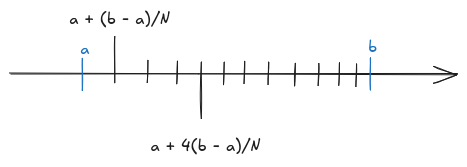
\includegraphics{../images/interval.png}

    Donc pour chaque intervalle on peut trouver un rationnels, on peut ensuite faire tendre N vers l'infini pour trouver un infinité de rationnels
\end{demonstration}

\begin{demonstration}
    D'apres notre démonstration précédente il existe un infinité de rationnels pour

    $a - \sqrt{2} \lt \dfrac{p}{q} \lt b - \sqrt{2} \implies a \lt \dfrac{p}{q} + \sqrt{2} \lt b$

    On en arrive avec la même logique que la démonstration précédente qu'il existe une infinité d'irrationnels entre deux réels.
\end{demonstration}
        
\section{Bornes sur $\R$}

\subsection{Maximum et minimum}

\begin{definition}
    Soit A une partie non vide de $\R$. Un réel M est le plus grand (resp. le plus petit) élément de A si $M \in A$ et
    $\forall x \in A, x \leq M$ (resp. $\forall x \in A, x \geq m$).

    Si il existe, le plus grand élément est unique et on le note max A.

    Si il existe, le plus petit élément est unique et on le note min A.
\end{definition}

\end{document}
